\chapter{Potatoes with Eggs}
\label{ch:eggswithpotatoes}
\index{eggs}
\index{potatoes}
\index{dinner}
\index{breakfast}

\marginnote{
    \textbf{Makes 4+ servings} \\
    Prep time: 15 hours \\
    Cook time: 20 minutes \\
    \vspace*{\baselineskip}

    Potatoes \\
    Eggs \\
    Olive oil \\
    Mitzithra or Pecorino romano, grated 
}

\textit{Patates me avga}

Family member: Grandma Elisavet

\newthought{Grandma Elisavet} would make \textgreek{πατάτες με αυγά} often for my dad and uncle when they were little. It was a meal that was easily put together and can sustain you for hours! Everytime we would visit our house in Dara, grandma would always have a place ready for us when we arrived because she knew we had travelled a long way and were hungry.

\begin{enumerate}
    \item Peel and cut the potatoes into wedges. Place them in a bowl of cold water.
    \item Heat a large frying pan, add some olive oil. When hot, add the potatoes and fry them. Once cooked, remove and set them aside on a plate.
    \item Add the eggs to the hot pan, mix them while they cook (scramble them). 
    \item As the eggs cook, add back the potatoes. Continue mixing with a spatula while the eggs cook.
    \item Put the potatoes and eggs onto a large place and sprinkle lots of grated cheese. Serve warm!
\end{enumerate}

% \begin{figure}
%   \includegraphics[width=60mm]{monanteras/images/Dara.pdf}
%   \caption{The House}
% \end{figure}
% \begin{figure}
%   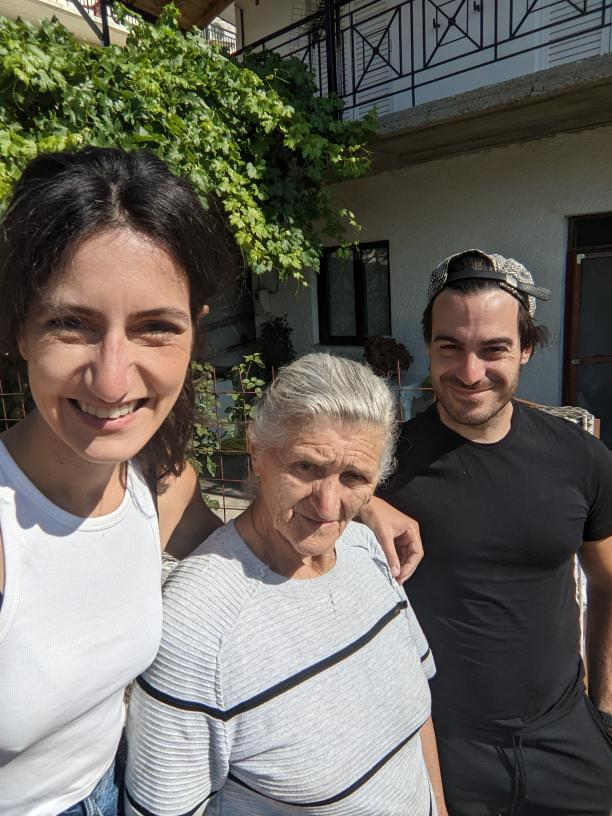
\includegraphics[width=60mm]{monanteras/images/Grandma elisavet.jpg}
%   \caption{In front of the house in Dara, Tripoli}
% \end{figure}

\twosidecaptionfigure{monanteras/images/Dara.pdf}{monanteras/images/Grandma elisavet.jpg}{(Left) The house, (Right) In front of the house in Dara, Tripoli}{fig:eggswithpotatoes}

